\section{Building the co-association matrix with different sparse formats}
\label{sec:spare building}

The purpose of this section is to present brief results concerning the time that took to build a co-association matrix for different types of matrices.
The ensemble from which the co-association matrices are built has 100 partitions and was produced from a mixture of 6 Gaussians with 5000 patterns.
Only the upper triangular (condensed) matrix was built.
The types of matrices under test are: fully allocated (a "normal" matrix), LIL, DOK, CSR, an optimized fully allocated and the proposed EAC CSR.
The SciPy's LIL, DOK and CSR implementations were used.
All tests were executed in machine Bravo.

The time that took to update the first partition and the total time were recorded for the different types of matrix.
The results are presented in Table \ref{tab:coassoc build sparse} and also in Fig. \ref{fig:coassoc build sparse}.
For the CSR format only the first partition was updated, since it took a very long time to update just the first partition.
A rough estimate for the time it would take to update the whole matrix is around 15 hours, 100 times the time it took to update the first partition.
Observing the other timings, and for the exception of the EAC CSR matrix, this estimate should not be too far off.
The reason that the first partition update of the EAC CSR matrix was so much faster is that it only requires a simple copy of the partition to the data structure.

It is clear from the results that the optimized versions are much faster than any of the others.
These results focus on providing a justification for the design and implementation of a novel method of building the co-association matrix: a fully allocated matrix consumes too much memory but available sparse implementations are too slow.
For this purpose a small dataset as the one used suffices to demonstrate this point.
The difference between the two optimized versions will become clearer on future sections, where a more thorough study covering a wider spectrum of datasets is presented. 


\begin{table}[h]
\centering
 \caption{Execution times for computing the condensed co-association matrix using different matrix strategies.}
\begin{tabular}{crr}
\toprule
  Matrix type (condensed) &  Time 1st partition [s] &  Time ensemble [s] \\
\midrule
 Optimzed Fully allocated &                 0.001 &              0.139 \\
                  EAC CSR &                 0.004 &              1.470 \\
          Fully allocated &                 0.855 &             96.000 \\
                      LIL &                 5.390 &            614.000 \\
                      DOK &                12.500 &           1535.000 \\
                      CSR &               548.000 &                - \\
\bottomrule
\end{tabular}
\label{tab:coassoc build sparse}
\end{table}



\begin{figure}[hbtp]
\centering
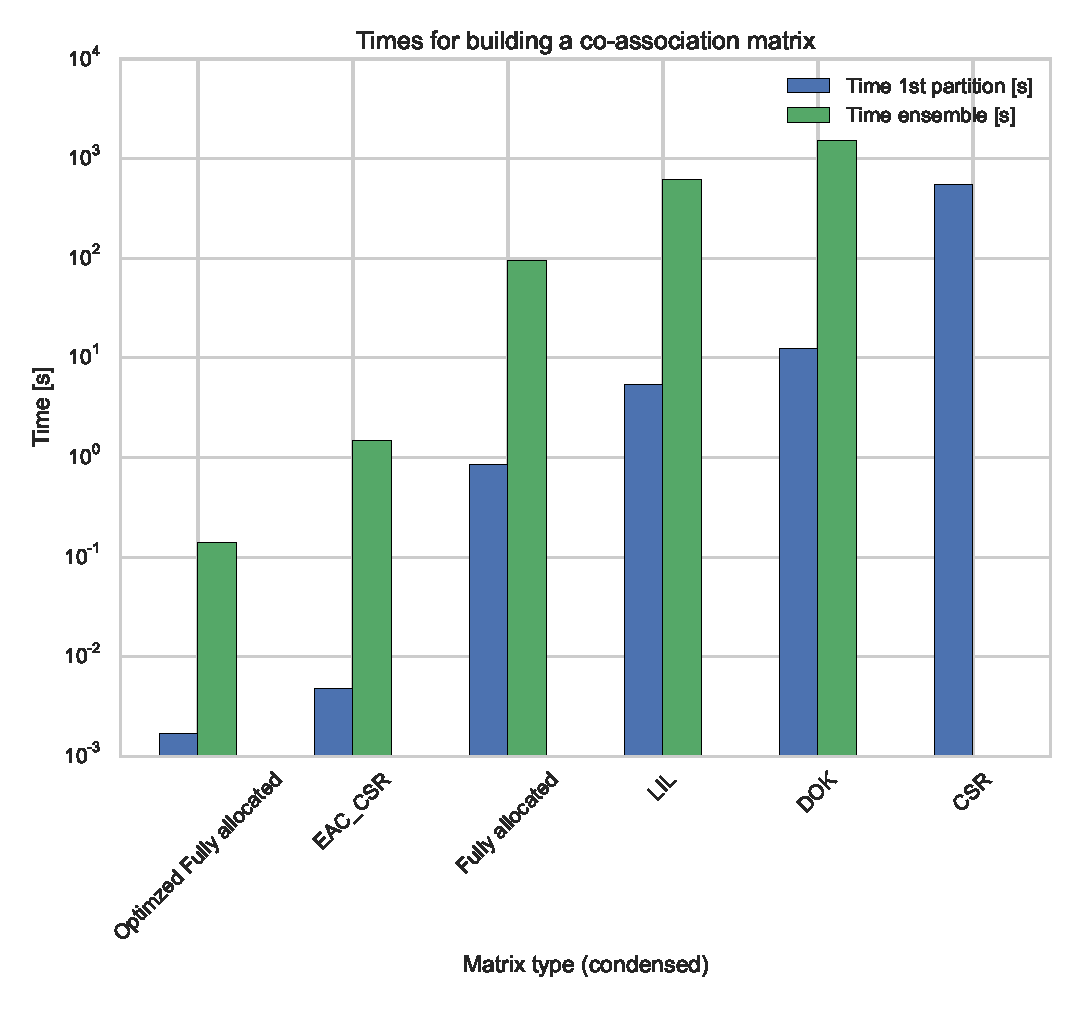
\includegraphics[scale=0.6]{results/eac_sparse_build/coassoc_build_bar}
\caption{Execution times for computing the condensed co-association matrix using different matrix strategies.}
\label{fig:coassoc build sparse}
\end{figure}